\documentclass[12pt]{article}    
\usepackage{ucs} 
\usepackage[utf8x]{inputenc}
\usepackage[russian]{babel}  
\usepackage{float}
\title{Псевдоэксперимент №2}
\author{Хафизов Фанис}
\usepackage[pdftex]{graphicx}
\usepackage{multirow}
\usepackage{mathrsfs}

\begin{document}
	\begin{figure}
		\centering
		
\includegraphics[width=0.3\linewidth]{logo}
	\end{figure}
	\maketitle
	\newpage
	\section{Движение без магнитов}
	Построим график зависимости $h_1(h_0)$ для легкого и тяжелого грузов.
	\begin{figure}[H]
		\centering
		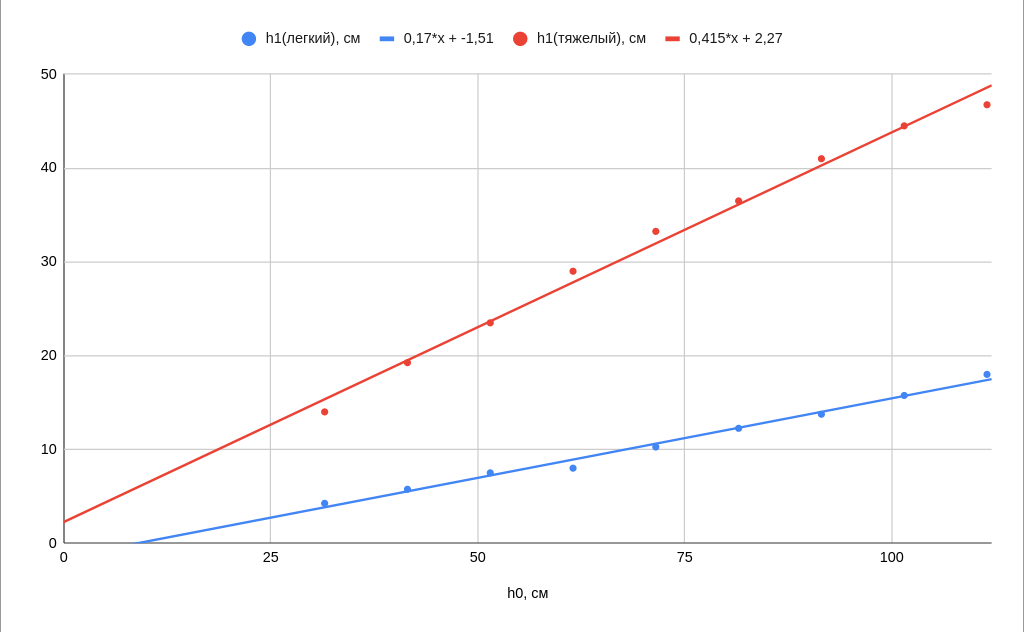
\includegraphics[width=\linewidth]{graph1}
		\caption{График зависимости $h_1(h_0)$ при отсутствии магнитов}
	\end{figure}
	Заметим, что зависимости имеют линейный характер. Можем предположить, что основная потеря энергии происходит в момент изменения направления вектора скорости в нижней точке траектории. При этом теряется фиксированная часть энергии, из-за чего отношение начальной и конечной высот постоянно. Силой трения воздуха можно пренебречь, так как скорость грузиков мала и зависимости линейны.
	\section{Магнитное торможение}
	Вновь построим графики зависимости $h_1(h_0)$ для обоих грузов
	\begin{figure}[H]
		\centering
		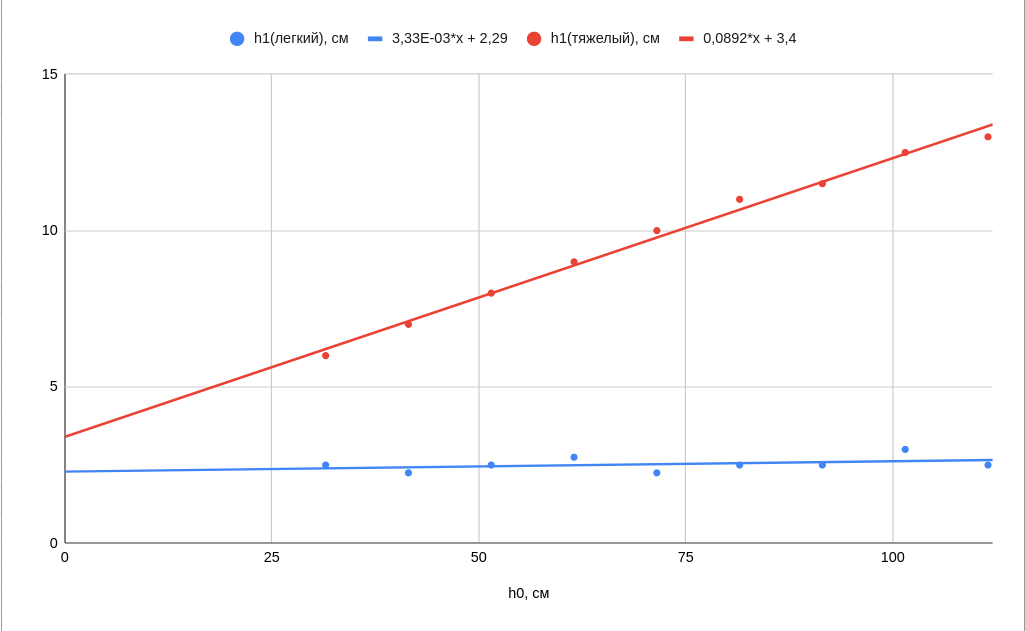
\includegraphics[width=\linewidth]{graph2}
		\caption{График зависимости $h_1(h_0)$ при вязком трении}
	\end{figure}
	Заметим, что снова графики линейны, но теперь у более легкого грузика $h_1=const$ вне зависимости от $h_0$. Это можно объяснить тем, что у легкого груза устанавливается скорость, и в нижней точке у него одинаковая скорость вне зависимости от начальной высоты. А значит, что он каждый раз будет подниматься на одинаковую высоту. Тяжелый же грузик не успеет достичь установившейся скорости, из-за чего его график возрастает.
	\section{Индукция магнитного поля магнита}
	Построим график зависимости $t(S)$.
	\begin{figure}[H]
		\centering
		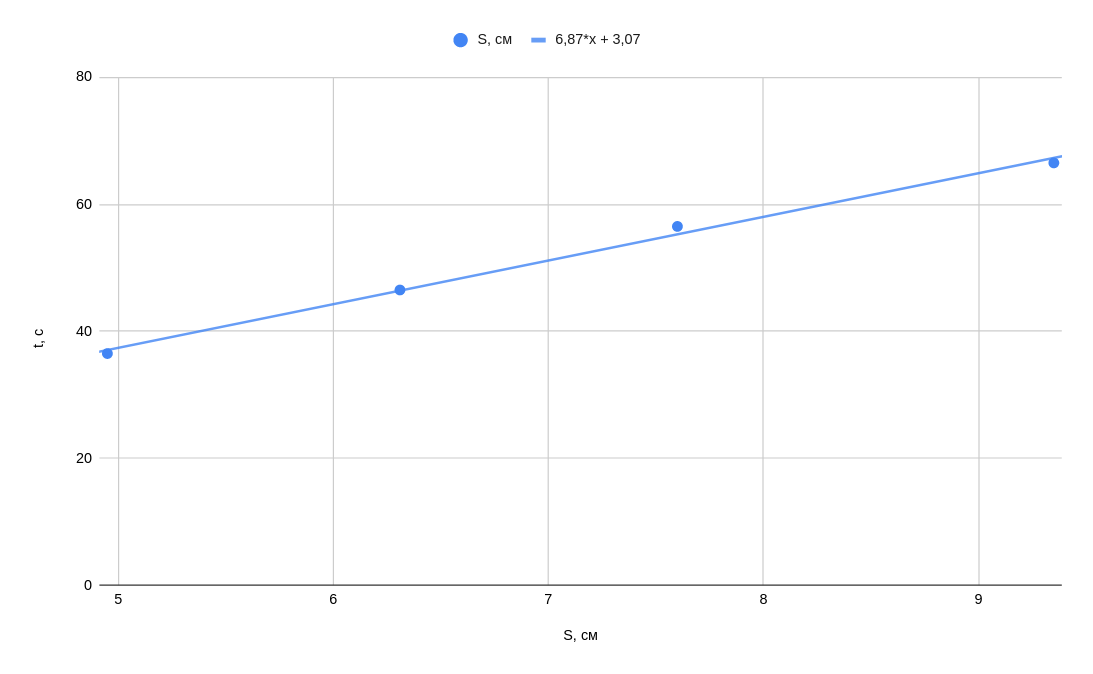
\includegraphics[width=\linewidth]{graph3}
		\caption{График зависимости $t(S)$}
	\end{figure}
	Полученный график имеет линейный вид. Это значит, что движение происходило с установившейся скоростью, то есть движение можно считать установившимся.\\
	$$M_{Fa} = F_a \cdot l_{Fa} = B I l \cdot l_{Fa} \sim B I \sim B \mathscr{E} = B \cdot (-\frac{d\Phi}{dt}) = B \cdot (-\frac{d(B\cdot S)}{dt})=-B^2\frac{dS}{dt} \sim B^2 \cdot v$$
	$$M_{Fa} = M_{T} = T\cdot l_T = mg\cdot l_t = const$$
	$$M_{Fa} = \alpha B^2 v$$
	$$B^2 v = mg\cdot l_t/\alpha$$
	$$v = S/t$$
	$$B^2/t = mg\cdot l_t/(\alpha S) = \beta$$
	$$B_1^2 / t_1= \beta$$
	$$B_2^2 / t_2= \beta$$
	$$B_3^2 / t_3= \beta$$
	$$B_1^2 / t_1 = B_2^2 / t_2 = B_3^2 / t_3$$
	$$B_1 = B_2\sqrt{\frac{t_1}{t_2}} = B_2\cdot0,822$$
	$$B_3 = B_2\sqrt{\frac{t_3}{t_2}} = 1,349B_2$$
	$$B_1 + B_2 = (1 + 0,822)B_2 = 1,822B_2$$
	$$B_3 \neq B_1+B_2$$
	Принцип суперпозиции не выполняется, так как когда мы взяли 2 пары магнитов значение их суммарной магнитной индукции не равно сумме значений индукций по отдельности.\\
	Так может быть из-за того, что часть силовых линий магнитной индукции не проходят через пластину, то есть, из-за краевых эффектов.
\end{document}